\section{Related Work}

\paragraph{Large Language Models}
Scaling up transformer-based language models in terms of model size, training data, and training compute has been shown to predictably improve performance on a wide range of downstream NLP tasks \citep{vaswani2017attention, devlin2018bert, brown2020language}. Many emergent abilities \citep{wei2022emergent} of LLMs have been discovered as a result of this scaling, including few-shot in-context learning, zero-shot problem solving, chain of thought reasoning, instruction following, and instruction induction \citep{cobbe2021training, wei2022chain, kojima2022large, sanh2022multitask, wei2021finetuned, ouyang2022training, honovich2022instruction}. In this paper, we view LLMs as black-box computers that execute programs specified by natural language instructions and investigate how to control an LLM's behavior using model-generated instructions. 

\paragraph{Prompt Engineering}
Prompting offers a natural and intuitive interface for humans to interact with and use generalist models such as LLMs. Due to its flexibility, prompting has been widely used as a generic method for NLP tasks \citep{schick2021exploiting, brown2020language, sanh2022multitask}. However, LLMs require careful prompt engineering, either manually \citep{reynolds2021prompt} or automatically \citep{gao2021making, shin2020autoprompt}, as models do not seem to understand the prompts in the same way a human would \citep{webson2021prompt, lu2021fantastically}. Though many successful prompt tuning methods perform optimization over a continuous space using gradient-based methods \citep{liu2021gpt, qin2021learning,lester2021power}, this becomes less practical with scale, as computing gradients becomes increasingly expensive and access to models shifts to APIs that may not provide gradient access. 
In our paper, we borrow components from discrete prompt search methods, such as prompt generation \citep{gao2021making, ben2021pada}, prompt scoring \citep{davison2019commonsense} and prompt paraphrasing \citep{jiang2020can, yuan2021bartscore} to optimize instructions by searching directly in the natural language hypothesis space. 
As compared to this past work, which uses specialized models for each component and leans heavily on human templates, we show that the entire search can be conducted by a single LLM.

\paragraph{Program Synthesis} Program synthesis involves the automatic search over a ``program space'' to find a program satisfying a particular specification \citep{gulwani2017program}. 
%Although classical program synthesis assumed a formal specification, this view has relaxed significantly and
Modern program synthesis admits a wide variety of specifications, including input-output examples \citep{ellis2021dreamcoder,wong2021leveraging} and natural language \citep{jain2022jigsaw}. The range of feasible program spaces to search over has also grown, from historically restrictive domain-specific languages to general-purpose programming languages \citep{austin2021program}. In contrast to prior approaches that require a suitable structured hypothesis space and library of components \citep{liang2010learning, ellis2018learning}, we leverage the structure provided by LLMs to search over the space of natural language programs. 
Using inference models is a standard practice to speed up the search by restricting the search space to a limited space of possible expressions  \citep{menon2013machine, lee2018accelerating, devlin2017neural, ellis2021dreamcoder}. 
Inspired by this, we use LLMs as approximate inference models to generate program candidates based on a small set of demonstrations. Unlike classical program synthesis, our inference models do not require any training and generalize well to various tasks.

\workshoponly{
\begin{figure}
  \centering
  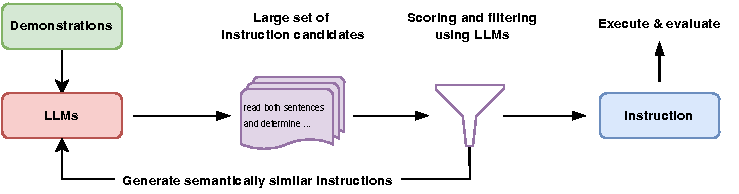
\includegraphics[width=0.8\linewidth]{figures/illustration/APE_pipeline.pdf}
  \caption{Our method, \textbf{Automatic Prompt Engineer (APE)}, automatically generates instructions for a task that is specified via output demonstrations: it generates several instruction candidates, either via direct inference or a recursive process based on semantic similarity, executes them using the target model, and selects the most appropriate instruction based on computed evaluation scores.}\label{fig:pipline}
\end{figure}
}